\documentclass[10pt,letterpaper,oneside]{article}
\usepackage{silence}
\usepackage{listings}
\WarningFilter{hyperref}{Token not allowed}    
\usepackage[T1]{fontenc}
\usepackage[latin1]{inputenc}
\usepackage[letterpaper,margin=2.5cm]{geometry}
\usepackage{amssymb,graphicx}
\usepackage[colorlinks=true,linkcolor=blue,citecolor=blue,filecolor=blue,urlcolor=blue]{hyperref}
\usepackage{etoolbox}
\makeatletter
\patchcmd{\chapter}{\if@openright\cleardoublepage\else\clearpage\fi}{}{}{}
\makeatother
\usepackage{parskip}


%%%%%%%%%%%%%%%%%%%%%%%Fonts%%%%%%%%%%%%%%%%%%%
\DeclareFontFamily{T1}{lmtt}{} 
\DeclareFontShape{T1}{lmtt}{m}{n}{<-> ec-lmtl10}{} 
\DeclareFontShape{T1}{lmtt}{m}{\itdefault}{<-> ec-lmtlo10}{} 
\DeclareFontShape{T1}{lmtt}{\bfdefault}{n}{<-> ec-lmtk10}{} 
\DeclareFontShape{T1}{lmtt}{\bfdefault}{\itdefault}{<-> ec-lmtko10}{} 

%%%%%%%%%%%%%%%%%%%%%%%Abbreviations%%%%%%%%%%%%%%%%%%%
\newcommand{\bnmr}{$\beta$-\textsc{nmr}}
\newcommand{\bnmrg}{\texttt{BNMR}}
\newcommand{\bnqr}{$\beta$-\textsc{nqr}}
\newcommand{\triumf}{\textsc{triumf}}
\newcommand{\cmms}{\texttt{CMMS}}
\newcommand{\isac}{\textsc{isac}}
\newcommand{\nmr}{\textsc{nmr}}
\newcommand{\musr}{$\mu$\textsc{sr}}

%%%%%%%%%%%%%%%%%%%%%%%IT%%%%%%%%%%%%%%%%%%%
\newcommand{\cpp}{\texttt{C++}}
\newcommand{\qt}{\texttt{QT}}
\newcommand{\minuit}{\texttt{MINUIT}}
\newcommand{\mud}{\texttt{MUD}}
\newcommand{\xmgr}{\texttt{Xmgr}}
\newcommand{\acegr}{\texttt{ACE/gr}}
\newcommand{\name}{\texttt{qtFit}}
\newcommand{\gsl}{\texttt{GSL}}
\newcommand{\qcp}{\texttt{QCustomPlot}}
\newcommand{\package}{\texttt{qtfit.tar.gz}}
\newcommand{\github}{\texttt{https://github.com/hsaadaoui/qtfit}}
\newcommand{\sourceforge}{\texttt{https://sourceforge.net/projects/qtfit/files/qtfit.tar.gz/download}}
\newcommand{\myemail}{\texttt{\href{mailto:saadaoui@triumf.ca}{saadaoui@triumf.ca}}}


%%%%%%%%%%%%%%%%%%%%%%%Text%%%%%%%%%%%%%%%%%%%%
\newcommand{\mycite}[6]{\bibitem{#1}#2 \etal, #3 {\bf {#4}}, {#5} ({#6}).}
\newcommand{\equ}[2]{\begin{equation}\label{#1}{#2}\end{equation}}
\newcommand{\meq}[2]{\begin{eqnarray}\label{#1}{#2}\end{eqnarray}}
\newcommand{\figs}[2]{Fig. \ref{#1}-(#2)}
\newcommand{\fig}[1]{Fig. \ref{#1}}
\newcommand{\etal}{{\it et al.}}
\newcommand{\ie}{{\it i.e.}}


\title{\name\ Documentation}
\author{Hassan Saadaoui \\
%\small{TRIUFM, 4004 Wesbrook mall, Vancouver, BC V6T~1Z4} \\
\small{\myemail}}
\date{\today}

\begin{document}

\maketitle

\begin{abstract}
 \noindent \normalsize
 \name\ is a program used to fit 	ASCII data.
 The  graphical user interface (GUI) of \name\ is designed using \qt\ software. 
 The regression is done using CERN's \minuit\ routine and plotting
 is perfomed with the \qcp\ library. 
 This document is a manual of the \name\ program, and includes 
 instructions about installation, features description, 
 and how-to-use examples.

\end{abstract}
\tableofcontents
\pagebreak


% =============================================================================== 

\section{Introduction}
\name\ is used to search, view, and analyze ASCII data. It can be extended by the user to read any type of data. This program is developed by Hassan Saadaoui and is maintained as needed. It is open source and released under the General Public License (GPL). No warranty or guarantee of the results is implied. Please acknowledge the author if you are using this program. For any questions, please email at \myemail.
\begin{figure}[!htb]
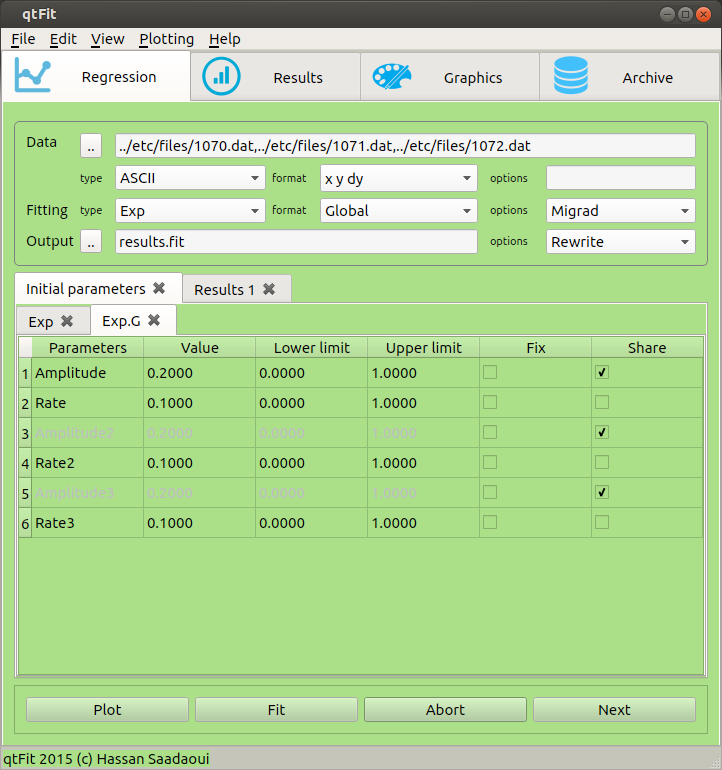
\includegraphics[width=\textwidth]{regression.png}
 \caption{Regression page of the \name\ graphical user interface.}
 \label{fig-dep}
 \end{figure}
\pagebreak


% =============================================================================== 

 \section{Requirements and structure}
The program is written in \cpp\ and \qt. The latter is used for general programming as well as the graphical user interface.  Version 4.8.x or 5.x is needed. The regression is done using \minuit\ minimization routine developed
at CERN. This package is originally in Fortran and later converted to \cpp. 
It is very powerful and well tested. \qcp\ library (included within the package) is used for data visualization. In addition to the above requirements, and depending on your system, you may also need other packages such as \texttt{gcc} compiler, and \texttt{automake}. The \name\ package contains 3 sub-folders and 5 files.
\begin{itemize}
 \item \verb+src/+: contains the source code, and includes the shared \verb+main.cpp+, and 
 \verb+mainwindow.(cpp,ui,h)+ and a sub-folder for each page.
 \item \verb+fct/+ contains the fitting functions and the script "\verb+compile+"
 to execute the codes and create the libraries.
 \item \verb+etc/+ for documentation, images, data, scripts
and templates, and the resources.qrc file needed by \qt.
 \item \verb+qtfit.pro+ used to generate the makefile.
 \item  \verb+AUTHOR+ for authorship attributions.
 \item \verb+COPYING+ supplies the GPL agreement.
 \item \verb+README.md+ for installation instructions.
 \end{itemize}

% =============================================================================== 

\section{Installation}
% =============================================================================== 
\subsection{\qt}
You need to install \qt\ 4.X.X or \qt\ 5.x binary and source packages.
Download the \qt\ on-line installer from \url{http://www.qt.io/download-open-source/}. 

% =============================================================================== 
\subsection{\minuit}To compile, do the following steps.
\begin{enumerate}
 \item  Download latest Minuit2 located at\\
\url{http://seal.web.cern.ch/seal/snapshot/work-packages/mathlibs/minuit/release/download.html}
 \item Unpack and cd
          \verb+$ tar -xvf minuit.tar.gz -C ~/+\\
          \verb+$ cd ~/minuit+
 \item  To install follow the instructions at
\\   \url{http://seal.web.cern.ch/seal/snapshot/work-packages/mathlibs/minuit/gettingStarted/autoconf.html}

 \item  Make SURE that the tests in the tutorial are running as described in the link \\ 
 \url{http://seal.web.cern.ch/seal/snapshot/work-packages/mathlibs/minuit/gettingStarted/testOutput.html}
  \item Copy (as superuser) the miniut libraries from   \\
  \verb+minuit/src/.lib/liblcg_Minuit.*+ to \verb+/usr/lib/+ \\
  \verb+$ sudo cp minuit/src/.lib/liblcg_Minuit.* /usr/lib/+
  \item Update ldconfig\\
 \verb+$ sudo ldconfig+
\end{enumerate}

{\bf Extra notes}: It is somewhat a challenge to compile Minuit2. These extra notes maybe useful.
\begin{itemize}
 \item Depending on your system, you may need to modify few codes namely  src/MnUserTransformation.cpp to add  \verb+#include <cstdio>+ or  \verb+#include <cstdio.h>+ just below  \verb+#include <algorithm>+ and re-compile.

 \item Locate where libraries and header files are, hopefully in  
 \verb+/usr/local/include/Minuit2+, and \verb+/usr/local/lib/+

 \item Add the path \verb+/usr/local/lib/+ to \verb+/etc/ld.so.conf+ as described here
 \url{http://stackoverflow.com/questions/1099981/why-cant-python-find-shared-objects-that-are-in-directories-in-sys-path}\\
 \\ \verb+$ export LD_LIBRARY_PATH=/usr/local/lib+ \\ or
 \\ \verb+$ export LD_LIBRARY_PATH=/usr/local/lib:$LD_LIBRARY_PATH+

 \item Run ldconfig
 \\ \verb+$ sudo ldconfig+
\end{itemize}


% =============================================================================== 
\subsection{\name}
\begin{enumerate}
 \item Download the latest \name\ from local computers, sourceforge, or github.\\
\verb+$ wget+ \sourceforge
 \item  Unpack it  \\     \verb+$tar -xvf+ \package\ \verb+-C ~/+
 \item  cd to the downloaded package
  \\  \verb+$ cd ~/qtfit+

 \item  If \qt\ binaries are not in your path, set the env (locate where qmake is)
\\    \verb+$ PATH=/usr/Qt/5.4/gcc_64/bin:$PATH + (change \verb+"/usr/Qt/5.4/gcc_64/bin"+ as per your system)
 \\   \verb+$ export PATH+

 \item  Run qmake
\\   \verb+$ qmake+

 \item  Run make and make install (as root)
 \\ \verb+$ make+
 \\ \verb+$ sudo make install+

 \item cd to directory \verb+fct/+ and compile all the libraries using the script compile
\\ \verb+$ cd fct+
\\   \verb+$ sudo ./compile+

 \item  To test the gui, invoke
\\  \verb+$ qtfit+
\\   or
\\  \verb+$ ./qtfit+ if not installed as root.
\end{enumerate}


% =============================================================================== 

\newpage
\section{Description of the GUI} 
The GUI has a menu bar at the very top and a tab widget below it. 
This tab widget contains 4 tabs (pages): \verb+Regression+, \verb+Results+, \verb+Plotting+, and \verb+Archive+. 
Each of these contains widgets for user  input and push buttons for issuing signals. 
The menu bar and the pages functionalities will be described next.
\subsection{Menu bar}
\begin{figure}[!htb]
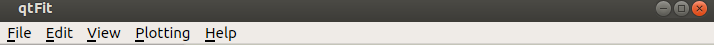
\includegraphics[width=\textwidth]{menubar.png}
 \caption{Menubar of the GUI.}
 \label{fig-mag}
 \end{figure}
{\bf File} has 2 options; (i) invoke a new window, and (ii) quit/close the window.

{\bf Edit} is empty for now, not finished...zzz.

{\bf View} to change the widget type of the GUI (default is \verb"fuse"+), 
and its color (default is \verb+"Green-white"+).

{\bf Plotting} not finished...zzzz.% where the user could check the box \verb+"Combine Plots"+. 

{\bf Help} This contains the \verb+"About"+ dialog for authorship and version of the current GUI,  \verb+"Tips"+ dialog which does nothing but remind the user that by hovering the mouse index onto labels one can get the tool-tips for each widget. \verb+"Tutorial"+ invokes an HTML page with these instructions.
	

% =============================================================================== 

\subsection{Regression}

\subsubsection*{Data input}
\begin{figure}[!htb]
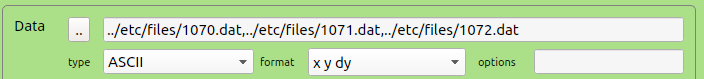
\includegraphics[width=\textwidth]{dataline.png}
 \caption{Data input of the regression page.}
 \label{fig-mag}
 \end{figure}
The user can choose to fit either ASCII text data or something else, for now it is only ASCII. The user can locate the data using the tool button next to Data for ASCII files. 
The data file must reside in the working directory, otherwise its full name with path should be given.
Filenames of the data to fit should be either given in the lineEdit (direct method); or using a file of \verb+.list+ or \verb+.inf+ suffix, and the user specifies the name of this file (eg: example.list or example.inf) in the lineEdit.  
\begin{itemize}
\item Direct input, the user can write in the lineEdit "Data" something like \verb+"file1.txt,file2.txt,file3.txt"+
\item Indirect input, the user can write in the lineEdit "Data" something like \verb+example.list+, and this file has nothing but a single ascii line like \verb+"file1.txt,file2.txt,file3.txt"+
\item Indirect input, the user can write in the lineEdit "Data" something like \verb+example.inf+, and this file contains the columns\\
\verb+filenames year variable+\\
\verb+file1.txt 2015 100+\\
\verb+file2.txt 2014 200+\\
\verb+file3.txt 2015 300+\\
\end{itemize}

The inner format of the ASCII file must be set in the field \verb+format+. The file must be in column format separated by space and no other characters than numbers. The limits of xmin and xmax values can be set in the options (settings) field. These must be numbers separated by commas.




% =============================================================================== 


\subsubsection*{Fitting selection}
\begin{figure}[h]
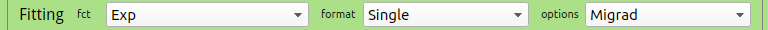
\includegraphics[width=\textwidth]{analyze-fct.png}
 \caption{Fitting functions input.}
 \label{fig-mag}
 \end{figure}

The user can select the function to use, the mode of fitting (single or global) and type of errors. The functions are defined in the folder \verb+fct/+ and the user can add new ones by invoking the selection \verb+"Create New"+ in the functions comboBox. The user must follow the instructions in the pop-up window and then select \verb+"Update"+ from the comboBox. This will add the newly defined function to the list. 

For the global method the user can choose to show all parameters for each run or not. These settings can be changed by double clicking on the initial parameters tab-widget. 

The errors are defined by \minuit\ routine, and are symmetric (Migrad) or asymmetric (Minos) errors. The latter are heavy to compute and the program may become unresponsive for sometime while the computation is ongoing. For further details read \url{http://seal.web.cern.ch/seal/documents/minuit/mnerror.pdf}.

% =============================================================================== 

\subsubsection*{Results output}
\begin{figure}[!htb]
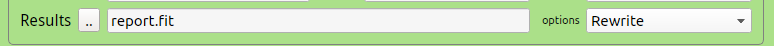
\includegraphics[width=\textwidth]{analyze-res.png}
 \caption{Fitting results output.}
 \label{fig-mag}
 \end{figure}
The fitting results are written to this file. The user must specify a name, or browse for an old file. The results can be either appended
 (using \verb+Append+) to the old file keeping its content (useful for doing run by run fitting), or the old file is overwritten using \verb+Rewrite+.

% =============================================================================== 

\subsubsection*{Parameters input}
\begin{figure}[!htb]
\center
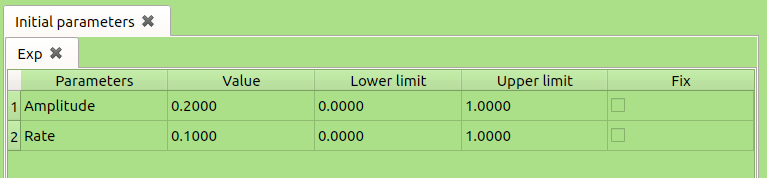
\includegraphics[width=.9\textwidth]{analyze-table-s.png}
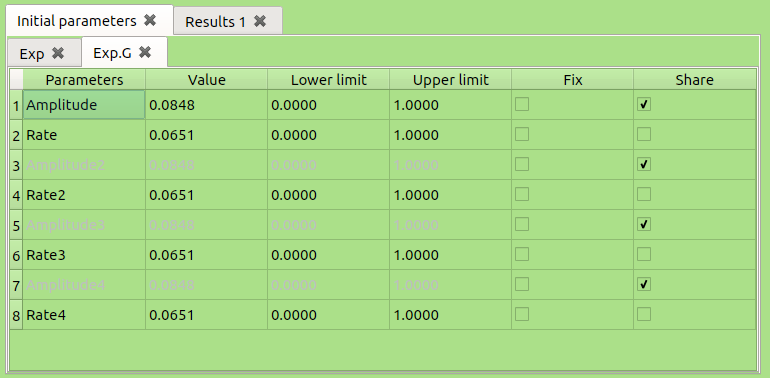
\includegraphics[width=.9\textwidth]{analyze-table-g.png}
 \caption{Input parameters for (a) single and (b) global fits. (a) The fit starts from this table for each file, or from the results of the last file in the sequence enabled by double clicking on the \texttt{"initial parameters"}. (b) If a parameter is shared between files, only the parameter of the first run is active and the same parameter for other files becomes inactive.}
 \label{fig-tables}
 \end{figure}
The initial parameters are read from the function library.
The table contains 5 columns for the single method, and 6 columns for the global method. These columns are; (1) parameter name, (2) initial value of the parameter, (3) lower limit, (4) upper limit, (5) fix the parameter checkBox, and (6) share the parameter checkBox.

These parameters can be changed, and saved in a template for future use  by right-clicking on the specific table and then choose \verb+"save as a template"+. This creates a text file template with a prefix \verb+".tab"+. The  user can change this text file as required, and the template can be loaded later for a similar function.

% ===============================================================================
\subsubsection*{Parameters output}
\begin{figure}[!htb]
\center
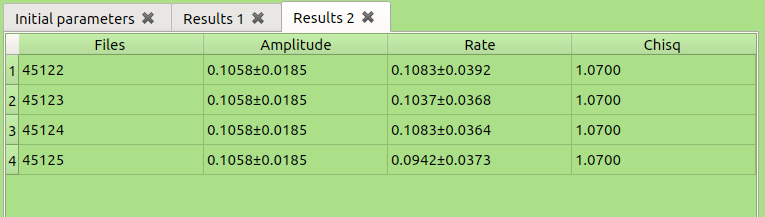
\includegraphics[width=.9\textwidth]{analyze-res-g.png}
 \caption{Results of a global fit where the shared parameter is Amplitude.}
 \label{fig-tables}
 \end{figure}
This prints out the output of the fit. The number of significant figures can be set by double-clicking on the results tab. One can also change the number of errors to show, and the way the filename is displayed.

% ===============================================================================
\subsubsection*{Input and output options}
The window shown in figure \ref{fig-top} can be invoked by double clicking on the 
header of the parameters table. In the pop-up window, the 
user can choose to show the parameters for all files in the case of a global fit, or 
use a common template for all files. The user can also choose to start the fit with the results of
best fitting parameters of the previous file in the sequence (only valid for single fit).
For the output table, the user can choose the format of the filename label,
parameters precision, and number of errors to display. 
\begin{figure}[!htb]
\center
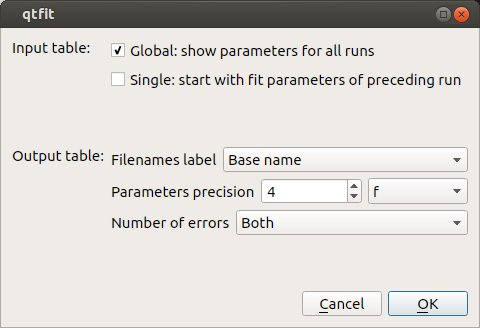
\includegraphics[width=0.5\textwidth]{tableoptions.png}
 \caption{Input and output options.}
 \label{fig-top}
 \end{figure}


% ===============================================================================
\newpage
\subsection{Results}
This page reads the files of fitting parameters created by the
analysis page. It displayed a table with two columns, the left column represents the x-axis and the right column the y-axis. Each column contains all fields found in the specified file (as created during the fitting).

The user can check any of the fields, and a matrix of plots of y versus x will be displayed.  The user can clear all choices using \verb+"Clear"+, and kill/delete the active table using \verb+"Purge"+. 

The plots will be displayed on the Graphics page. Horizontal or vertical error bars are displayed if specified in the chosen parameter. 

\begin{figure}[!htb]
\center
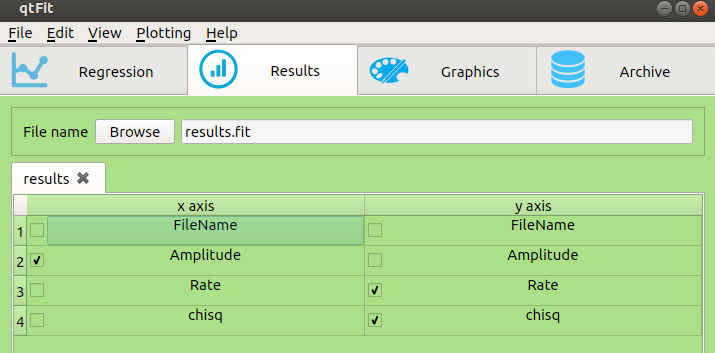
\includegraphics[width=\textwidth]{resultstop.png}

\includegraphics[width=\textwidth]{resultsbottom.png}
 \caption{Results page snapshots.}
 \label{fig-results}
 \end{figure}



% =============================================================================== 



\newpage
\subsection{Graphics}
The plots of the regression page and results pages are displayed here.
The user can \verb+export+ the graphs into png or pdf, or \verb+Purge/Clear+ (delete) 
the active window(s), or go the archive database with \verb+Next+.
\begin{figure}[!htb]
\center

\includegraphics[width=\textwidth]{graphics.png}
 \caption{Graphics page.}
 \label{fig-results}
 \end{figure}


% =============================================================================== 

\newpage
\subsection{Database}
This page offers a user-friendly interface for databases, and
uses SQLite language \url{http://www.tutorialspoint.com/sqlite/sqlite_overview.htm}. At the start, the user must select a database by clicking on the toolButton next to \verb+"Database"+, or create a new one from the \verb+"Querry"+ lineEdit using SQL commands and hitting \verb+"Execute"+.
It is advised to use an SQL manager (like the friendly browser extension SQLite manager) to create databases and tables. Then, one can use this interface to add/delete rows and edit cells, interact with the content of the database. But an experienced user can do everything from this page as well by executing the \verb+"Querry"+ commands.
Te get familiar with the interface, \verb+"physics.sqlite"+ is supplied. 
Each contain several tables. The user can load any of these tables from the comboBox, 
and a model of the table will be displayed. 

The user can execute any query to study the loaded table. Example;\\ \verb+SELECT * FROM table_of_constants where Unit="kg"+ will select all fields in the \verb+table_of_constants+ where the unit is in kg. The user must be familiar with SQL to execute from the Query field. Any table can be changed by adding or deleting rows. Also each cell can be edited, or displayed by clicking on \verb+"Open"+. This can be used to display a cell with a lot of text or view the cell as image if the full path of the image was given in that cell. 
\begin{figure}[!htb]
\center
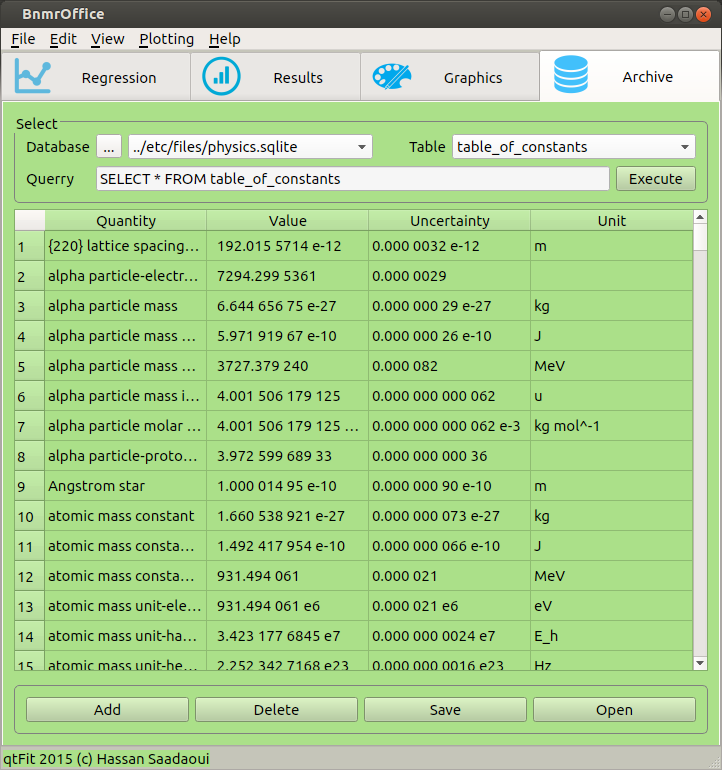
\includegraphics[width=0.8\textwidth]{archive.png}
 \caption{Database interface loaded with a table of physical constants.}
 \label{fig-mag}
 \end{figure}



% =============================================================================== 

\newpage
\section{Fitting functions}
The user can write his own fitting functions in the directory \verb+fct/+.
A new function must be written in \cpp\ but requires minimal programming knowledge of this language. 
At template of a typical function is as follows:
%\begin{verbatim}
\begin{lstlisting}[language=C++, keywordstyle=\color{red}]
#include <iostream>
#include <fstream> 
#include <math.h>
#include <stdio.h>
#include <vector>
#include <sstream>   
#include <string.h>
#include <iostream>
using namespace std;
#include "parameters.h"

//Wrap in "C" for the compiler.
extern "C" 
{ 
  //The defalt initial parameters loaded to the table.
  void defaultParameters(Parameters &defaults)
  {
    defaults.addParameter( "Amplitude" , 0.2, 0.001, 0.15, 1.0 );//par[0]
    defaults.addParameter( "Rate"      , 0.1, 0.001, 0.0,  1.0 );//par[1]
  }
  //This must have the same number of parameters as in the default parameters above.
  double function(double x, const std::vector<double> par)
  {
  	return par[0]*exp( - par[1]*x);//par[0] is amplitude and par[1] is rate.
  }
}
\end{lstlisting}
%\end{verbatim}
The user must follow these instructions:
\begin{itemize}
\item Make a copy of the file \verb+newFunction.cpp+ found in \verb+qtfit/etc/files+.
\item Rename the file (eg: newfct.cpp) and save it in the folder \verb+qtfit/fct/+.
\item cd to the directory \verb+qtfit/fct/+, and run the script "\verb+compile+"" as root\\\
 \texttt{$\$$ sudo ./compile name}   (eg: sudo ./compile newfct.cpp)
 \end{itemize}
This compiles the library and puts a copy in the functions folder (\verb+/usr/local/qtfit/fct/+).


% =============================================================================== 

\newpage
\section{How-To-Use examples}
\subsection{Example 1}
\begin{enumerate}
\item After the installation is complete, open the \name\ program from a terminal using the command 
\verb+qtfit+.
\item Go to the page \verb+Regression+.
\item To load a data file, click on the toolButton next to the label \verb+"Data"+. 
Browse the directory \verb+qtfit/etc/files+ and load the files \verb+1070.dat+ to  \verb+1072.dat+,
(Hold-on Ctrl key to select more than one file). 
\item Select \verb+ASCII+ under "type" comboBox, and \verb+xydy+ under format.
Leave the \verb+Options+ field empty for now.
\item Under Fitting; select the function \verb+Exp+ (for exponential fit), and format \verb+Single+
(for single fits), and \verb+Migrad+ (symmetric errors) for the type errors.
\item Write an appropriate name for the output file, any name is acceptable, 
or leave it as default \verb+results.fit+.
\item Click on  \verb+Plot+ pushButton at the bottom of the page to plot and view the selected files.
\item Click on \verb+Fit+ pushButton at the bottom of the page to perform the regression. If the fit 
converges, the results of the fit will be displayed in a new table. Go to Graphics page to see the plots of
the raw data and fitting functions.
\item Click on \verb+Next+ to send the file  \verb+results.fit+ to the results page. The columns of this
file will be displayed, and the user can choose to plot a column against the other. On the left, check the box of 
\verb+Amplitude+ as x variable, and on the right-side of the table 
check the box \verb+Rate+ as y variable. Click on Plot, this will plot Rate versus Amplitude.
Go to the page Graphics to see the new plot.
If you click on \verb+Clear+ all checkboxes will be unselected. 
If you click on \verb+Purge+ all shown tables will be deleted.  
If you click on \verb+Next+ the Graphics window will be shown. 
\end{enumerate}

\subsection{Example 2}
\begin{enumerate}
\item To load a ".inf" file, click on the toolButton next to the label \verb+"Data"+. 
Browse the directory \verb+qtfit/etc/files+ and load the file \verb+example.inf+.
The header of this file looks like this:\\
\verb+#FileName              Time(min) Temperature(K)+\\
\verb+../etc/files/1070.dat  25        10,0.1+ \\
\verb+../etc/files/1071.dat  22        20,0.3+\\
In this example, the ".inf" file contains three colums defined in the header 
(preceded by the sign $\#$): the filename, a variable called Time in units of min, and 
a variable called Temperature in units of K. The arguments of each columns are given in the next rows.
For Temperature, the given value is accompanied by the error.  For example, "\verb+10,0.1+" means Temperature $= 10\pm0.1$ K for the file 1070.dat. In all columns (except the filename), 
the user can specify one or two errors (asymmetric),
and all numbers must be separated by a comma.  
For example, something like "\verb+88,0.1,0.2+" means Temperature $=[88-0.1,88+0.2]$ K.
\item Repeat steps 4 to 9 in example 1.
\end{enumerate}

\end{document}
